\documentclass{beamer}

\usepackage[utf8]{inputenc}
%\usepackage{beamerthemesplit}
\usepackage{url}
\usepackage{tikz}
\usepackage{alltt}
\usepackage{listings}
\usepackage{marvosym}
\usepackage{color}
\usepackage[multidot]{grffile}
\usepackage{multirow}
\usepackage{array}
\usepackage{setspace}
\usepackage{hyperref}
\usepackage{verbatim}
\usepackage{fancyvrb}
%\hypersetup{colorlinks=true, linkcolor=blue,  anchorcolor=blue,  
%citecolor=blue, filecolor=blue, menucolor=blue, pagecolor=blue,  
%urlcolor=blue} 
\lstset{keywordstyle=\bfseries\color{brown},
        stringstyle=\ttfamily,
        commentstyle=\color{blue}\textit,
        showstringspaces=false}

\useoutertheme{}
\usetheme{Madrid}
\graphicspath{{pics/}{global/}
{pics/I/}{pics/A1/}{pics/A2/}{pics/A3/}{pics/A4/}{pics/A5/}{pics/A6/}{pics/A7/}
}

\logo{
\includegraphics[height=1cm]{ProcessHorizontal}} 

\institute{Center for Computation and Technology\\Louisiana State University, Baton Rouge, LA}

\setbeamertemplate{navigation symbols}{} 

\title{CSC 7700: Scientific Computing}

% We want to use the infolines outer theme because it does not use a lot of
% space, but it also tries to print an institution and the slide
% numbers (which we might not want to show). Therefore, we here redefine the
% footline ourselfes - mostly a copy & paste from
% /usr/share/texmf/tex/latex/beamer/themes/outer/beamerouterthemeinfolines.sty
\defbeamertemplate*{footline}{infolines theme without institution and slide numbers}
{
  \leavevmode%
  \hbox{%
  \begin{beamercolorbox}[wd=.25\paperwidth,ht=2.25ex,dp=1ex,center]{author in head/foot}%
    \usebeamerfont{author in head/foot}\insertshortauthor
  \end{beamercolorbox}%
  \begin{beamercolorbox}[wd=.5\paperwidth,ht=2.25ex,dp=1ex,center]{title in head/foot}%
    \usebeamerfont{title in head/foot}\insertshorttitle
  \end{beamercolorbox}%
  \begin{beamercolorbox}[wd=.25\paperwidth,ht=2.25ex,dp=1ex,center]{date in head/foot}%
    \usebeamerfont{date in head/foot}\insertshortdate{}
  \end{beamercolorbox}}%
  \vskip0pt%
}

% Some useful commands
\newcommand{\abspic}[4]
 {\vspace{ #2\paperheight}\hspace{ #3\paperwidth}\includegraphics[height=#4\paperheight]{#1}\\
  \vspace{-#2\paperheight}\vspace{-#4\paperheight}\vspace{-0.0038\paperheight}}

\newcommand{\picw}[4]{{
 \usebackgroundtemplate{
 \color{black}\vrule width\paperwidth height\paperheight\hspace{-\paperwidth}\hspace{-0.01\paperwidth}
 \hspace{#4\paperwidth}\includegraphics[width=#3\paperwidth, height=\paperheight]{#1}}\logo{}
 \frame[plain]{\frametitle{#2}}
}}
\newcommand{\pic}[2]{\picw{#1}{#2}{}{0}}

\newcommand{\question}[1]{\frame{\frametitle{#1}
 \begin{centering}\Huge #1\\\end{centering}
}}


\documentclass{beamer}

\usepackage[utf8]{inputenc}
%\usepackage{beamerthemesplit}
\usepackage{url}
\usepackage{tikz}
\usepackage{alltt}
\usepackage{listings}
\usepackage{marvosym}
\usepackage{color}
\usepackage[multidot]{grffile}
\usepackage{multirow}
\usepackage{array}
\usepackage{setspace}
\usepackage{hyperref}
\usepackage{verbatim}
\usepackage{fancyvrb}
%\hypersetup{colorlinks=true, linkcolor=blue,  anchorcolor=blue,  
%citecolor=blue, filecolor=blue, menucolor=blue, pagecolor=blue,  
%urlcolor=blue} 
\lstset{keywordstyle=\bfseries\color{brown},
        stringstyle=\ttfamily,
        commentstyle=\color{blue}\textit,
        showstringspaces=false}

\useoutertheme{}
\usetheme{Madrid}
\graphicspath{{pics/}{global/}
{pics/I/}{pics/A1/}{pics/A2/}{pics/A3/}{pics/A4/}{pics/A5/}{pics/A6/}{pics/A7/}
}

\logo{
\includegraphics[height=1cm]{ProcessHorizontal}} 

\institute{Center for Computation and Technology\\Louisiana State University, Baton Rouge, LA}

\setbeamertemplate{navigation symbols}{} 

\title{CSC 7700: Scientific Computing}

% We want to use the infolines outer theme because it does not use a lot of
% space, but it also tries to print an institution and the slide
% numbers (which we might not want to show). Therefore, we here redefine the
% footline ourselfes - mostly a copy & paste from
% /usr/share/texmf/tex/latex/beamer/themes/outer/beamerouterthemeinfolines.sty
\defbeamertemplate*{footline}{infolines theme without institution and slide numbers}
{
  \leavevmode%
  \hbox{%
  \begin{beamercolorbox}[wd=.25\paperwidth,ht=2.25ex,dp=1ex,center]{author in head/foot}%
    \usebeamerfont{author in head/foot}\insertshortauthor
  \end{beamercolorbox}%
  \begin{beamercolorbox}[wd=.5\paperwidth,ht=2.25ex,dp=1ex,center]{title in head/foot}%
    \usebeamerfont{title in head/foot}\insertshorttitle
  \end{beamercolorbox}%
  \begin{beamercolorbox}[wd=.25\paperwidth,ht=2.25ex,dp=1ex,center]{date in head/foot}%
    \usebeamerfont{date in head/foot}\insertshortdate{}
  \end{beamercolorbox}}%
  \vskip0pt%
}

% Some useful commands
\newcommand{\abspic}[4]
 {\vspace{ #2\paperheight}\hspace{ #3\paperwidth}\includegraphics[height=#4\paperheight]{#1}\\
  \vspace{-#2\paperheight}\vspace{-#4\paperheight}\vspace{-0.0038\paperheight}}

\newcommand{\picw}[4]{{
 \usebackgroundtemplate{
 \color{black}\vrule width\paperwidth height\paperheight\hspace{-\paperwidth}\hspace{-0.01\paperwidth}
 \hspace{#4\paperwidth}\includegraphics[width=#3\paperwidth, height=\paperheight]{#1}}\logo{}
 \frame[plain]{\frametitle{#2}}
}}
\newcommand{\pic}[2]{\picw{#1}{#2}{}{0}}

\newcommand{\question}[1]{\frame{\frametitle{#1}
 \begin{centering}\Huge #1\\\end{centering}
}}



\subtitle[Module A]{{\large Module A: Basic Skills}\\*[0.3em]Lecture 4: Advanced 1D and 2D Visualization}
\author[\mbox{
\includegraphics[height=0.6em]{fl_300}\hspace{0.5em}Frank Löffler}]{Dr Frank Löffler}
\date{Fri, Sep 13 2013}
\titlegraphic{\hspace{3cm}
\includegraphics[height=0.5cm]{just_a_black_cat_by_dooftan-d4uqnzs}}
\usecolortheme[RGB={18,86,125}]{structure}

\begin{document}

\frame{\titlepage}

\section{Overview}
\frame{\frametitle{Overview}
 1D and/or 2D visualization
 \begin{itemize}
  \item Publications
  \item Debugging
  \item Quickly put together
  \item Does not require fast network connections if done remotely
 \end{itemize}
 3D visualization
 \begin{itemize}
  \item Web / PR (movies)
  \item Detailed Debugging
  \item Comparably slower to achieve than 1D/2D plots
 \end{itemize}
}

\frame{\frametitle{1D/2D tools}
 \abspic{MATLAB_mesh_sinc3D}{0.1}{0.5}{0.4}
 Common (biased):
 \begin{itemize}
  \item Gnuplot
  \item Matplotlib
  \item Supermongo (*)
  \item Tecplot (*)
  \item GNU Octave
  \item Grace
  \item Maple/Mathematica (*)
  \item Matlab (*)
  \item Maxima/Sage
 \end{itemize}
 (*): license necessary
}

\section{Matplotlib Overview}
\frame{\frametitle{}\begin{centering}\LARGE\insertsectionhead\\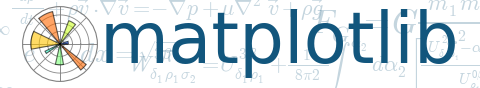
\includegraphics[height=2cm]{logo_matplotlib}\end{centering}}

\frame{\frametitle{Matplotlib}
 \begin{itemize}
  \item Python
   \begin{itemize}
    \item programming language
    \item high-level
    \item large and comprehensive standard library
    \item often used as scripting language
    \item available for a wide range of OSs
   \end{itemize}
  \item NumPy extension
   \begin{itemize}
    \item support for large, multi-dimensional arrays and matrices
    \item high-level math functions
   \end{itemize}
  \item SciPy extension
   \begin{itemize}
    \item linear algebra, integration, interpolation, special functions, FFT, signal and image processing, ODE solvers, ...
    \item data structures provided by Numpy
   \end{itemize}
  \item Interactive: pylab (closely resembles Matlab interface)
 \end{itemize}
}

\section{Matplotlib Examples}
\frame{\frametitle{}\begin{centering}\LARGE\insertsectionhead\\\end{centering}}

\frame{\frametitle{Hello World: plot sin(x)}
\begin{centering}
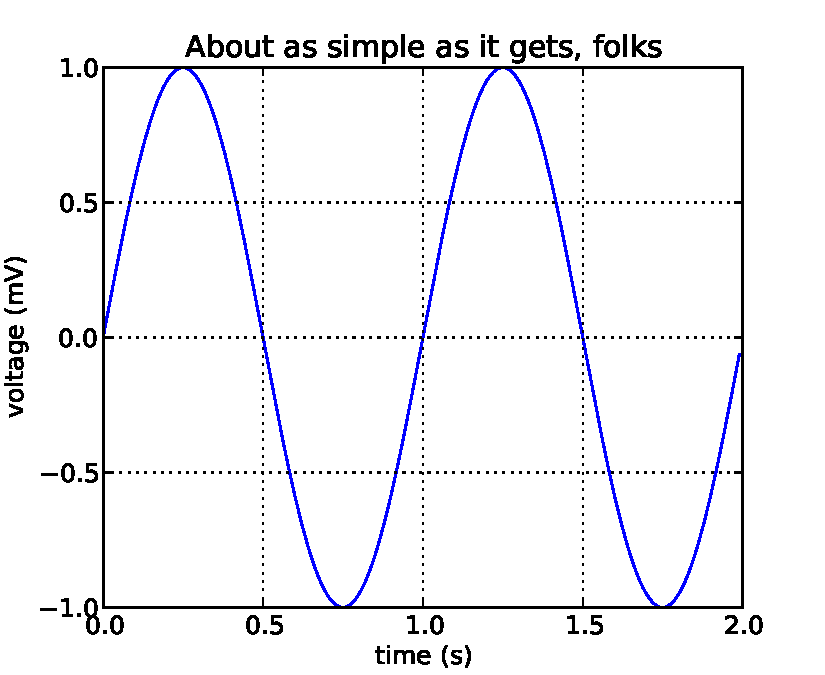
\includegraphics[height=8cm]{simple_plot}\\
\end{centering}
}

\frame[containsverbatim]{\frametitle{Hello World: plot sin(x)}
\abspic{simple_plot}{0.0}{0.6}{0.35}
\small\include{samplecode/A4/simple_plot}
}

\frame{\frametitle{Subplots}
\begin{centering}
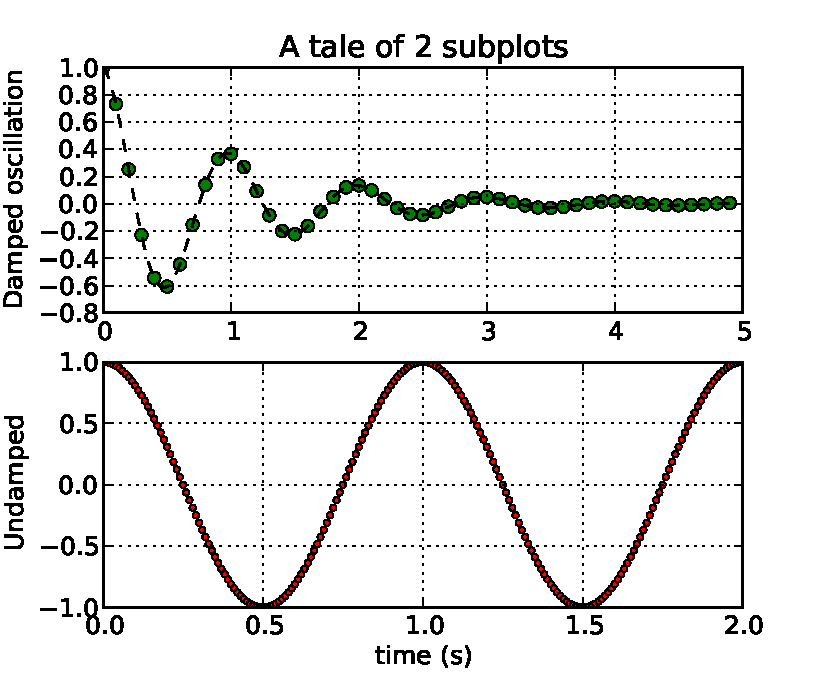
\includegraphics[height=8cm]{subplot_demo}\\
\end{centering}
}

\frame[containsverbatim]{\frametitle{Subplots}
\abspic{subplot_demo}{0.0}{0.6}{0.35}
\tiny\include{samplecode/A4/subplot_demo}
}

\frame{\frametitle{Histograms}
\begin{centering}
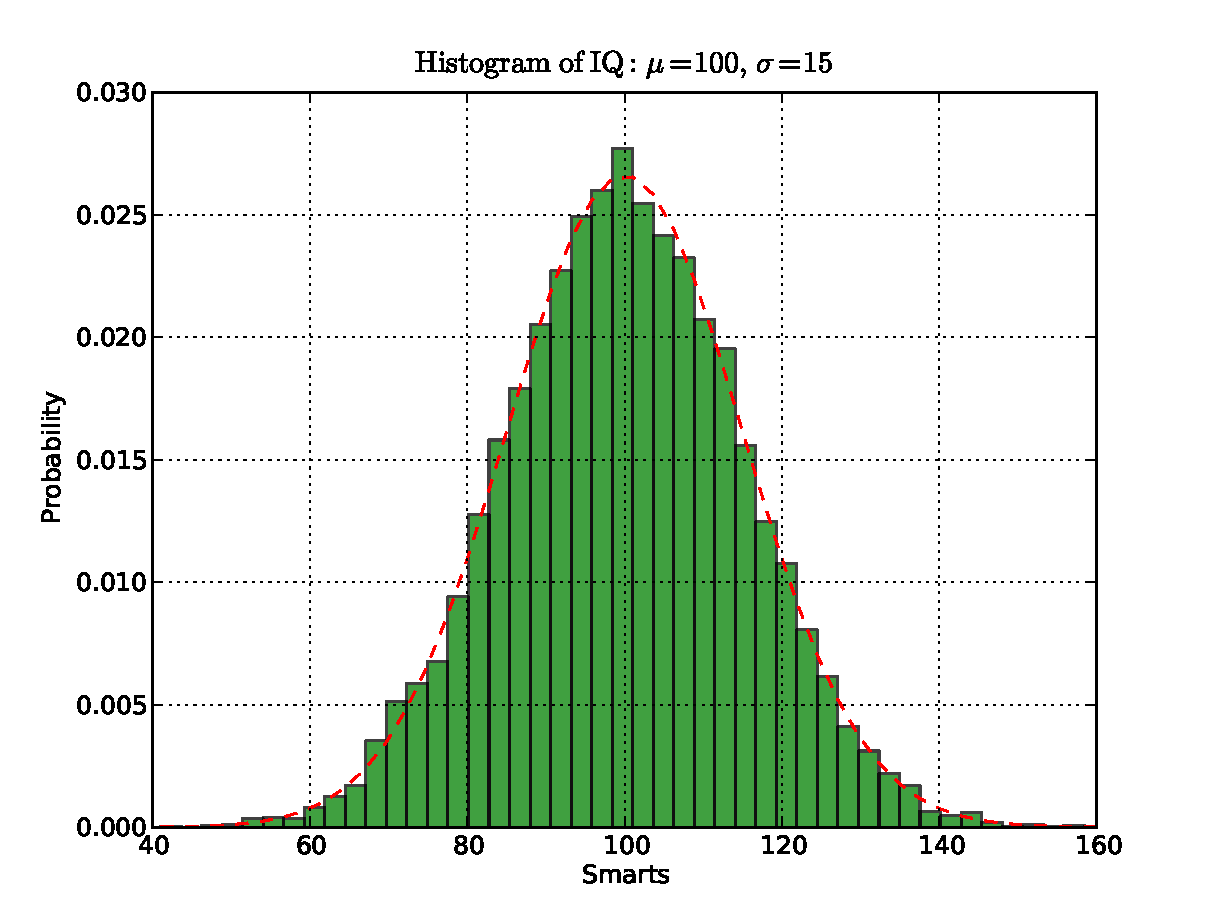
\includegraphics[height=8cm]{histogram_demo}\\
\end{centering}
}

\frame[containsverbatim]{\frametitle{Histograms}
\abspic{histogram_demo}{0.0}{0.6}{0.3}
\tiny\include{samplecode/A4/histogram_demo}
}

\frame{\frametitle{Surfaces}
\begin{centering}
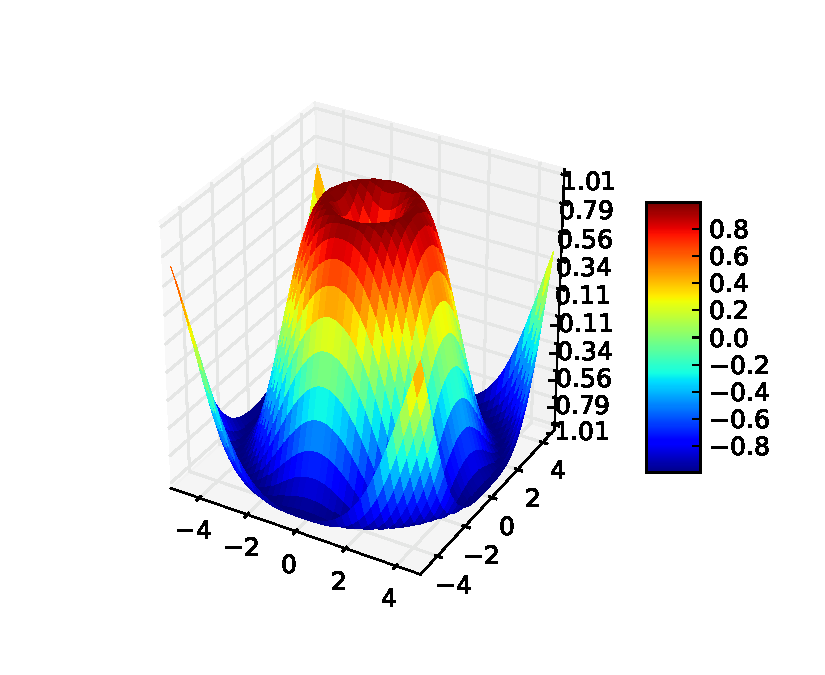
\includegraphics[height=8cm]{surface3d_demo}\\
\end{centering}
}

\frame[containsverbatim]{\frametitle{Surfaces}
\abspic{surface3d_demo}{0.0}{0.6}{0.35}
\tiny\include{samplecode/A4/surface3d_demo}
}

\frame{\frametitle{Log plots}
\begin{centering}
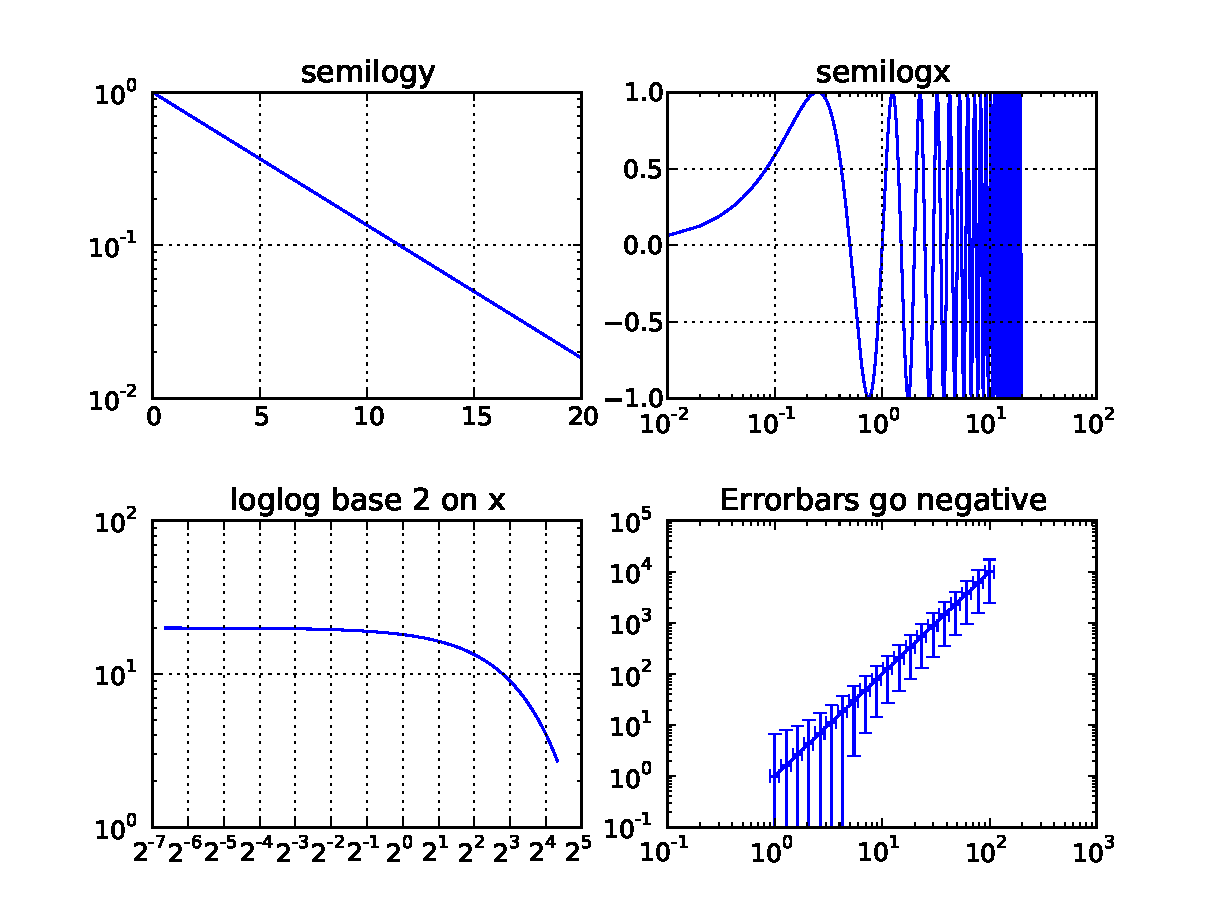
\includegraphics[height=8cm]{log_demo}\\
\end{centering}
}

\frame[containsverbatim]{\frametitle{Log plots}
\abspic{log_demo}{-0.08}{0.5}{0.4}
\begin{minipage}{0.45\linewidth}
\tiny\include{samplecode/A4/log_demo_1}
\end{minipage}
\begin{minipage}{0.45\linewidth}
\vspace{3cm}
\tiny\include{samplecode/A4/log_demo_2}
\end{minipage}
}

\frame{\frametitle{Legends}
\begin{centering}
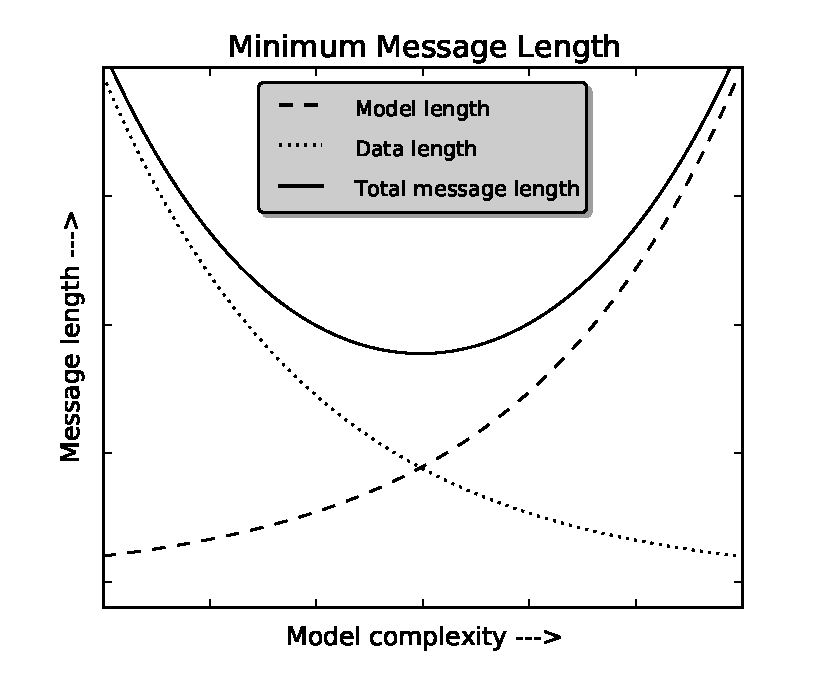
\includegraphics[height=8cm]{legend_demo}\\
\end{centering}
}

\frame[containsverbatim]{\frametitle{Legends}
\abspic{legend_demo}{0.0}{0.65}{0.3}
\begin{minipage}{0.42\linewidth}
\tiny\include{samplecode/A4/legend_demo_1}
\end{minipage}
\begin{minipage}{0.45\linewidth}
\vspace{3cm}
\tiny\include{samplecode/A4/legend_demo_2}
\end{minipage}
}

\frame{\frametitle{Native TeX rendering}
\begin{centering}
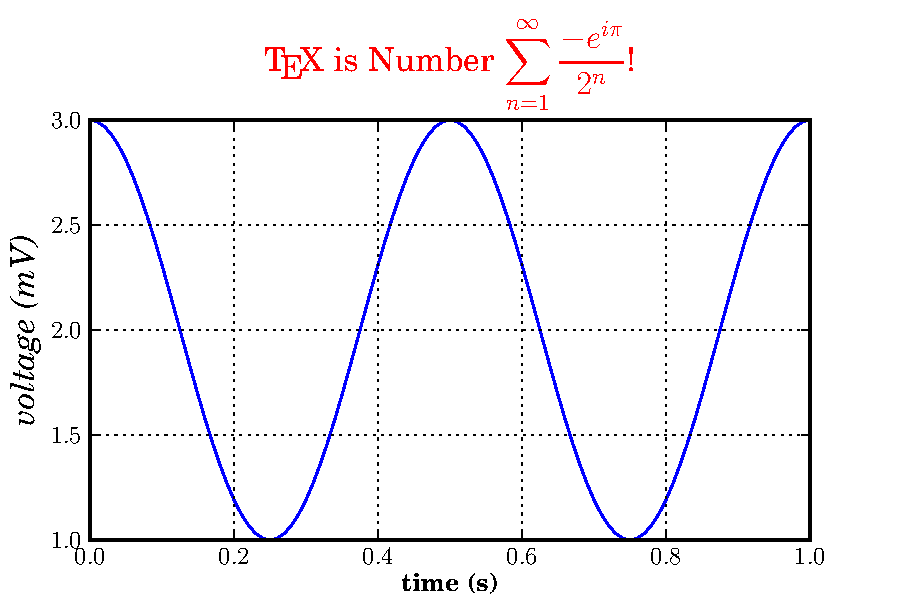
\includegraphics[height=8cm]{tex_demo}\\
\end{centering}
}

\frame[containsverbatim]{\frametitle{Native TeX rendering}
\abspic{tex_demo}{0.0}{0.6}{0.3}
\tiny\include{samplecode/A4/tex_demo}
}

\section{File Input}
\frame{\frametitle{}\begin{centering}\LARGE\insertsectionhead\\\end{centering}}

\frame[containsverbatim]{\frametitle{Text files}
\verb|data.txt|:
\verbatiminput{samplecode/A4/data.txt}
}

\frame[containsverbatim]{\frametitle{Text files - loadtxt()}
Note: Each row in the text file must have the same number of values\\
\abspic{loadtxt}{0.05}{0.67}{0.25}
\small\include{samplecode/A4/loadtxt}
}

\frame[containsverbatim]{\frametitle{Text files with missing columns}
\verb|data2.txt|
\verbatiminput{samplecode/A4/data2.txt}
}

\frame[containsverbatim]{\frametitle{Text files - genfromtxt()}
\abspic{loadtxt}{0.05}{0.67}{0.25}
\small\include{samplecode/A4/genfromtxt}
}


\frame[containsverbatim]{\frametitle{Production example}
\begin{centering}
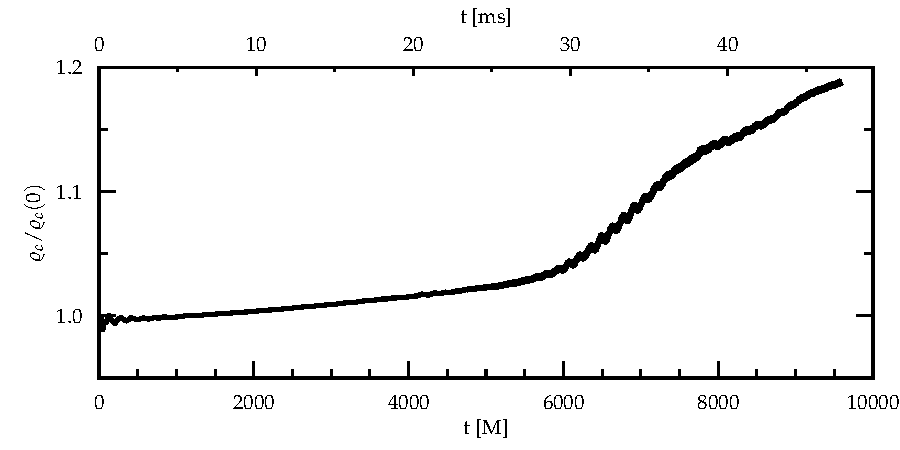
\includegraphics[height=6cm]{rho_max}\\
\end{centering}
}

\frame[containsverbatim]{\frametitle{Production example}
\abspic{rho_max}{0.05}{0.55}{0.25}
\tiny\include{samplecode/A4/rho_max}
}

\frame[containsverbatim]{\frametitle{Production example}
\abspic{rho_max}{0.05}{0.55}{0.25}
\tiny\include{samplecode/A4/plot_defaults}
}

\frame[containsverbatim]{\frametitle{Interactive Usage}
 \tiny
 \begin{verbatim}
$ ipython --pylab
Python 2.7.3 (default, Jan  2 2013, 13:56:14) 
Type "copyright", "credits" or "license" for more information.

IPython 0.13.1 -- An enhanced Interactive Python.
?         -> Introduction and overview of IPython's features.
%quickref -> Quick reference.
help      -> Python's own help system.
object?   -> Details about 'object', use 'object??' for extra details.

Welcome to pylab, a matplotlib-based Python environment [backend: TkAgg].
For more information, type 'help(pylab)'.

In [1]: x = randn(10000)

In [2]: hist(x,100)
 \end{verbatim}
}

\section{Course Work}
\frame[containsverbatim]{\frametitle{Course Work}
Use \href{https://svn.cct.lsu.edu/repos/courses/sci-comp-2013-public/coursework/A4/}
{template and data [1]} to create this plot, send Python source and pdf-file.\\
\begin{centering}
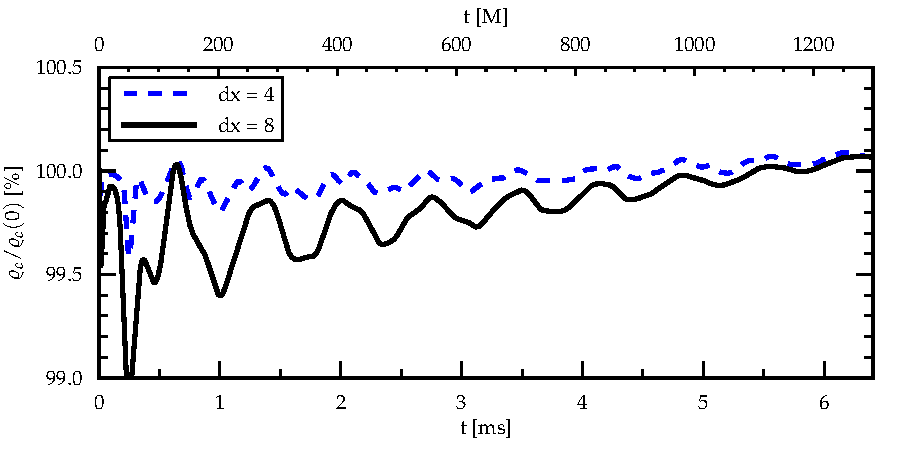
\includegraphics[height=6cm]{rho_max_coursework}\\
\end{centering}
\tiny{[1] \href{https://svn.cct.lsu.edu/repos/courses/sci-comp-2013-public/coursework/A4/}{https://svn.cct.lsu.edu/repos/courses/sci-comp-2013-public/coursework/A4/}}
}

\frame[containsverbatim]{\frametitle{Course Work}
Things to change from given example:
\begin{itemize}
 \item Plot data from two files in one plot, using line styles as in example
       (blue and dotted, black and solid)
 \item Switch the two $x$-axes and make sure they line up properly
 \item Add legend (key) as shown (length of lines not important)
 \item Show percentage on $y$ axis instead of raw quotient
 \item Add $[\%]$ to $y$-label
 \item Show ticks on y axes as in example
 \item Commit: python script, resulting pdf file, no full report (coursework/A4)
\end{itemize}
\vspace{2em}
\textbf{Due: Fri, Sep 20th 2013}
}

\end{document}

